\documentclass[onecolumn, draftclsnofoot,10pt, compsoc]{IEEEtran}
\usepackage{graphicx}
\usepackage{url}
\usepackage{setspace}
\usepackage{pdfpages}
\usepackage{lscape}
\usepackage[noadjust]{cite}  

\usepackage{geometry}
\geometry{textheight=9.5in, textwidth=7in}

% 1. Fill in these details
\def \CapstoneTeamName{		Project BoxSand}
\def \CapstoneTeamNumber{		6}
\def \GroupMemberOne{			Max Moulds}
\def \GroupMemberTwo{			Sam Morey}
\def \GroupMemberThree{			Anya Lehman}
\def \CapstoneProjectName{		Project BoxSand}
\def \CapstoneSponsorCompany{	Oregon State Physics Department}
\def \CapstoneSponsorPerson{		Dr. Kenneth Walsh}

% 2. Uncomment the appropriate line below so that the document type works
\def \DocType{		Design Document
				%Requirements Document
				%Technology Review
				%Design Document
				%Progress Report
				}
			
\newcommand{\NameSigPair}[1]{\par
\makebox[2.75in][r]{#1} \hfil 	\makebox[3.25in]{\makebox[2.25in]{\hrulefill} \hfill		\makebox[.75in]{\hrulefill}}
\par\vspace{-12pt} \textit{\tiny\noindent
\makebox[2.75in]{} \hfil		\makebox[3.25in]{\makebox[2.25in][r]{Signature} \hfill	\makebox[.75in][r]{Date}}}}
% 3. If the document is not to be signed, uncomment the RENEWcommand below
%\renewcommand{\NameSigPair}[1]{#1}

%%%%%%%%%%%%%%%%%%%%%%%%%%%%%%%%%%%%%%%
\begin{document}
\begin{titlepage}
    \pagenumbering{gobble}
    \begin{singlespace}
        \hfill 
        % 4. If you have a logo, use this includegraphics command to put it on the coversheet.
        %\includegraphics[height=4cm]{CompanyLogo}   
        \par\vspace{.2in}
        \centering
        \scshape{
            \huge CS Capstone \DocType \par
            {\large\today}\par
            \vspace{.5in}
            \textbf{\Huge\CapstoneProjectName}\par
            \vfill
            {\large Prepared for}\par
            \Huge \CapstoneSponsorCompany\par
            \vspace{5pt}
            {\Large\NameSigPair{\CapstoneSponsorPerson}\par}
            {\large Prepared by }\par
            Group\CapstoneTeamNumber\par
            % 5. comment out the line below this one if you do not wish to name your team
            \CapstoneTeamName\par 
            \vspace{5pt}
            {\Large
                \NameSigPair{\GroupMemberOne}\par
                \NameSigPair{\GroupMemberTwo}\par
                \NameSigPair{\GroupMemberThree}\par
            }
            \vspace{20pt}
        }

    \end{singlespace}
\end{titlepage}
\newpage
\pagenumbering{arabic}

\begin{abstract}
Project BoxSand is a online learning environment that is focused on bringing open educational resources to secondary education students. Currently the site maintains collection of Physics resources used by Dr. Kenneth Walsh to instruct a algebra based physics course at Oregon State University \cite{boxsand}. This development team is creating additional functionality for the project and transitioning the existing website to another web application framework with the specific goal to implement a homework system capable of assigning assessments based on reading or answering questions. 
\end{abstract}

\tableofcontents
% 7. uncomment this (if applicable). Consider adding a page break.
%\listoffigures
%\listoftables

\singlespacing
\section*{Date of Issue and Status}
1st of December 2017

\hfill \break
This document is subject to change and at the date and time listed above represents the best effort to fully represent the software design decision of the project following the IEEE-1016-2009 standard where appropriate.

\section*{Issuing Organization}
This document is written during the 2017-2018 Capstone cycle and is for the Project BoxSand Development team.  

\section*{Change History}
Change History
\newline
1 December 2017 Version 1.0


\clearpage


% 8. now you write!
\singlespacing

\section{Introduction}
\subsection{Purpose}
The purpose of this document is to serve as a guideline for development team of BoxSand for the 2017-2018 year. This document will be an evolving document and will change throughout the lifespan of development. Eventually the document  will also serve as a handy reference guide for future BoxSand development teams.

\subsection{Scope}
This document details the design plans for the BoxSand project. It entails details of the different viewpoints of the project as well as detailing the current plans for project implementation including the authorship and context of the project. Each viewpoint is specified by the design concerns and design elements of each viewpoint.

\subsection{References}
\bibliographystyle{IEEEtran}  
\bibliography{designdocument_6_final} 

\section{Body}
\subsection{Identification of the SDD}
We are using Agile/Lean with SCRUM as a basis for design patterns and for architectural patterns, the MVC model will be used. We are therefore choosing viewpoints and views with direct relation to those processes. This includes viewpoints from our stakeholders; users, developers and customers, and their views of each of our components as defined by our architecture.

\subsection{Stakeholders}
Stakeholders for the project include three groups: users, developers, and customers. The main stakeholder in this project is Dr. Kenneth Walsh of the Department of Physics at Oregon State University

\subsubsection{Users}
Users of the application have specific interfaces needs that change based on login credentials and usage intentions. Groups include students, instructors, content contributors, and administrators.

\subsubsection*{Students}
This group of users represents the majority of individual users of the application and are the main target for the use of the application. This is consistent with the project overarching goals defined further in the Problem Description Document. 

\subsubsection*{Instructor}
The instructor stakeholder requires the ability to change aspects of the application pertaining to associated content within a course maintained by the instructor. For this development cycle the information an instructor can incorporate in a course is limited to the information from the existing BoxSand website, OpenStax textbook hosted at \cite{openstax-book}, and the OpenStax question bank provided by CNX \cite{quadbase}.

\subsubsection*{Content Contributors}
Content contributors consist of users that add new content and reorganize existing content within the BoxSand site. This group differs from an instructor in that a member of this group does not associate with a course or have access to change those designs but instead can only add to the content offered by the application. For this development cycle, initial content is uploaded using a developer-base process and future content contribution systems will be considered in the design of required aspects of this development cycle. This design concern for this group of stakeholders dictates appropriate documentation detailing the use and operation of the systems providing the content for the application 
\subsubsection*{Administrators}
This group includes LAs, TAs, and site maintainers that are tasked with day to day operation of the deployed application and other operations required by the customer. For this development cycle, this group has design requirements that are included in this cycle while actual development requirements and implementation are not included in this 2017-2018 cycle. 
\subsubsection{Developers}
The developer user group consists of entities required to maintain the application outside of day-to-day operation and include future feature implementation, mitigating integrity issues, and providing long-term maintainability. The design concerns for this group consist of application fit criteria and mostly pertain to maintainability, integrity, and ensuring future interoperability. 
\subsubsection{Customer}
The customer stakeholder represents the design considerations that satisfy the research needs for the project. Since BoxSand also incorporates the data collection mechanisms for research conducted by Dr. Walsh where the relationship between student success and site interaction is studied. 
\subsection{Design Concerns}
Project design concerns are summarized in the SRS and the Problem Statement document. In the following sections, this design document will detail considerations of these concerns as they relate to specific software components utilized by the application and development process.

\section{Design Views}

\subsection{Web Application Framework}
As stated in earlier in the SRS and the Problem Description, many choices regarding web application framework implementations were made to keep project development in alignment with partners. Regardless of that constraint, Rails is an appropriate solution to build the underlying framework for the application. Other software considerations are referenced in the Technical Review document dealing with this component.

\subsubsection{Design View}
Rails is a collection of components written in the programming language Ruby and are used to implement web applications. Rails use many pre-built components to help development progress more quickly and make assumptions about the way a developer wants to implement aspects of a application \cite{rails-mvc}. 
\begin{figure}
 \centering 
  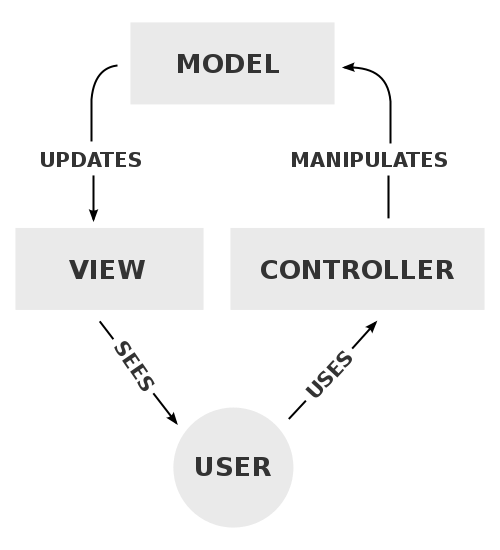
\includegraphics[scale=0.4]{MVC-Process.png}\cite{mvc-image}
\end{figure}
Rails provides the structure for the individual components and is not technically a single feature. Instead, Rails provides a framework for managing other software components detailed in a manifest file. When a project is begun in Rails, software dependencies and components referred to as gems are listed in a manifest file and that file is used by a specific gem called bundler that builds the application dependencies along with other some other things. 

\subsubsection{Design Overlays}
Using a configuration of Rails from a partner project requires the development team to use restrictions imposed by that partner. OpenStax is currently updating many components of their software to reduce technical debt and update dependencies which can require the development team to do the same. Rails, in its current fifth version, specifies Ruby 2.2.1 as a base language, however the OpenStax applications mostly require Rails version 4.2 and a Ruby version of 2.2.3 and are transitioning to the 2.4.2 version of Ruby \cite{rails-version}.

\subsubsection*{Non-Rails}
Since this application does not squarely fit entirely into a Rails application some ancillary software components need to be configured to interface with a Rails applications. Components included in these non-Rails configured dependencies are managed by other various mechanism and are partly enumerated in the Dev Guide and deployment scripts. 

\subsubsection*{Node}
Future versions of the application will have to work with the alternative to Rails, Node. The client has expressed strong desires to implement features that require Node and therefore it must be considered in the design now. This caveat may be a useful tool for developers in this cycle that are struggling with the steep learning curve associated with Ruby and the wide availability of support documentation for Node solutions. Building the application with both Node and Rails operating in tandem is a solution that should not be completely excluded. 

\subsubsection{Design Rationale}
\subsubsection*{Criteria}
Any framework chosen must interface with the other components chosen by the development team and be able to be used to meet client goals. Assessing the quality of a potential component is not as simple as comparing a set list of features provided, but also involves considering the long term outlook for any software component and its fit with past code and other partner contributions. In addition to satisfying the technical requirements, a major deciding factor in any comparison between comparable components is the use of the component by our partners. Since the existing application uses components that are not compatible with the application being developed all new choices pose interesting implications such as longevity, availability of support, maintainability and generally the need to address any sunk cost in development caused from transitioning from one major software component to another. An example in this project arises with the deprecation of Drupal, a mostly standalone PHP based content management system, and the implementation of a more dynamic and capable yet complex system using the OpenStax framework. This change of components is also not one-to-one since transitioning to OpenStax will ultimately require the use of Nginx, Apache, Rails, and Node to interoperate together. 

\subsubsection*{Rails}
Using a web application framework designed with emphasis on rapid development is import to this development team for this cycle because many of the features that require implementation will be completed in a shorter timeframe than future development iterations due to the increased amount of initial documentation and research. Moving forward with Rails over the other option Node, minimizes differences between this project and partner projects which will lessen the need for maintenance in the long term. Rails is a stable component for the project and shows promising long term viability but is growing at a slower rate than the alternative solution. The complexities of the decision to use Rails continue to grow as client expectations change and interoperability requirements update to reflect partner restrictions. An example of this growing source of complexity is the issue of portability and standards compliance specifically if the project is expanded and other entities are included such as Canvas. Further compounding this issue is the fact that many components of future features are already implemented using aspects of both Rails and Node. 

\subsection{User Interface}
The frontend, or the user interface, refers to the way that the user will interact with the webpage and how they get the knowledge of how to correctly use the services provided by a the site. Through the user interface the user can retrieve information from the system and input changes to the system. The main design concern of the User Interface is that it needs to be easy for a student to quickly understand how to use. The goal is to make the students life as easy as possible, and reduce the total amount of navigation around the site.  The more straightforward the user interface the better for the student's learning. The user interfaces that will need to be developed are the landing page for the site, the user dashboard for both the student and the instructor user types, and the pages that contain the course content. The design of the user interface will be written in CSS language. CSS applies design decisions to all of the items in a class format to insure that similar items are displayed in the same way. 

\subsubsection{Design View}
The main tool that will be used for user interface development will be Sketch. Sketch is a vector graphics editor that can connect with several plugins to help design the user interface.\cite{sketch} With the use of Sketch, it will be possible to create the design plan for the user interface without the need to grapple with code. After the design is created, Sketch can pull out the CSS code needed to turn the design into software. Thiss CSS can then be applied over the user interface to make sure that items in the user interface are consistently recognizable  to the user.

\subsubsection{Design Overlays}
Using Sketch requires that we have access to a Mac operating system. This is potentially an issue for contributors who do not own a mac computer. This will put limitations on when user interface development can be made by members of the project who do not have regular access to a mac computer or a mac operating system virtual machine.
\subsubsection{Design Rationale}
The use of a user interface design software is important because it will allow for design decisions to be made before interface code is written and implemented. Since code can be harder for a person to interpret, changes to design ideas are harder to make in code form. With the use of a interface development tool, design ideas can be quickly created, and tweaked to find an interface that will be best for the user.  If this were to be attempted in a programming language first, time will need to be dedicated to figuring out how to code an idea for each idea rather than simple taking that time at the end once a design has been decided upon. 


\subsection{User Tracking}
User Tracking specifically refers to the following things to track: ability to track clicks including time and date of click, time spent on a webpage, and time spent watching a video. BoxSand tracks this data so that research can be done on student's behavior and how it correlates to success. JavaScript and an appropriate framework such as Angular will be used to accomplish this task. It should be noted that this section will be slightly vague, because the Project BoxSand team is still working on how this portion of the project will be developed. Additionally to all of this information Project BoxSand's primary stretch goal is to implement a annotation/highlight system on the textbook portion of the website. This would allow students to converse about the textbook through comments on highlighted sections. 
\subsubsection{Design View}
JavaScript frameworks are a tool for making JavaScript easier to manage. It provides premade tools for making websites easier to develop, and allows for a more readable code base. Beyond this there are even prebuilt libraries such as Angulartics that can be used that are made for the specific kind of tracking that Project BoxSand requires. 
\subsubsection{Design Overlays}
Using a framework requires that Project BoxSand be designed in the style of that particular framework. This is not inherently bad, but it does put limitations on the overall design of the project. In addition to this frameworks create dependencies, while the overall benefits from frameworks outweigh their downsides, it still increases complexity of the overall application. 
\subsubsection{Design Rationale}
Use of a framework is important for Project BoxSand because it helps speed up the process of development, and for a short development cycle of a few months this is vital. 

\subsection{Data Storage}
The components used by this project impose strict data storage requirements on data required and generated by the project and application. Constraints exist that limit the options the development team are allowed to implement. For instance certain legal requirements, discussed at greater length in the SRS, require that data gathered from the application be stored separately from grade and student information and that grade data used in rendering user dashboards must be handled with escalated levels of privacy controls. Conversely, the requirement forces the development team to meet exceedingly higher levels of compliance when dealing with privileged data and content. This requirement also mandates extensive testing and will need more time in development due to that process. Selecting a inadequate component to handle the data storage for the project would have large consequences on the effectiveness of the development team. For this development cycle, the decisions of the partners regarding data storage has been mirrored by the development team almost verbatim. Even though there exists a strong motivation to stay within the familiar components used by the partners of the project, alternative solutions for this component should be explored and compared to the adopted components from the development partners. Detailing the features needed by the data engine and storage system show that the application needs the ability to store large collections of highly fragmented and often incomplete data as seen with user interaction data. This dataset will also need to be completely copied regularly to be digested by the research group associated with the project. 
\subsubsection{Design View}
PostgreSQL is a object-relational database management system. PostgreSQL is ACID compliant, transactional, supports views, triggers, foreign keys, and is designed around 5 years lifespans. The downside to Postgres is that few in the development team have explicit experience with it. Another downside to Postgres is the relative unfamiliarity of the development team with the specifics of this component. The Postgres data engine manages account data, both sensitive client and user data and insensitive generated data. The assessment database is also provided by Postgres and requires a custom configuration per deployment. Many other entities that interface with CNX and OpenStax assume Postgres as the data engine and for that reason the development team decided to continue using Postgres as the data engine solution. The other appropriate option supported by the partners is MySQL but only minimal time was spent assessing the completeness of a solution using MySQL as the data engine.  Aside from standard uses and configuration, which are non-issues, the data engine Postgres is being used by multiple components which each provide part of the complete data set required. Documentation of these component dependent configurations is minimal or non-existent so there has not been any considerable development time invested in exploring the replacement of the data engine. 
\subsubsection{Design Overlays}
\subsubsection*{Assessments}
One of the most important aspects of the project is the client specified feature of being able to assign homework questions from both the OpenStax textbooks and the OpenStax database of assessments or questions. Access to the OpenStax assessments are not as straightforward as the textbook and require interfacing with CNX, another entity associated with OpenStax. Outside of the collection of homework and other questions hosted by CNX, there are no real benefits for this project to partner with this entity. Instead, a one-time collection of these resources has been decided as the best procedure given our development constraints. This reduces complexity but also stagnates the content on BoxSand and is to be addressed in future development cycles. The assessment database from CNX requires special interactions with seldomly used components of OpenStax and some components that are not required by the BoxSand project at all. The data storage engine for the project must be able to be adapted to serve as a replacement to the CNX content source once the content has been ported to the project data storage.
\subsubsection{Design Rationale}
OpenStax uses two data storage solutions: PostgreSQL and Redis. The Technical Review document details the decision to use the two in greater depth but a summary of that analysis found that Redis would be used to store derivative data generated by secondary components not directly related to the primary goals of this project, including the adaptive learning already existing in the OpenStax framework. This is not needed immediately by our project. For Postgres, the decision is less clear. OpenStax has made an effort to remove the need for a specific data engine used by their components which leads the development team to make the generalization that the data engine is loosely coupled to the functionality of partner components, or at least it is realistic to consider replacing the data engine later in development. The design of future features must address the long term ramifications of using Postgres as the data engine. Since it is supported by the source of hardware used to provide base system used by the partners project but is not a specific limitation of our development group, this team should explore advantages to changing data engine when possible.

\subsection{Container Host}
While a container host was not a specific requirement of out client, it is still an important part of the development process and will be included here for that reasons. The container host is  important because it allows the development team to keep the development process streamlined. This is an indirect requirement brought about by the shortened timeframe for initial development. Keeping a clean and easily deployable development environment, while not directly related to client requirements, indirectly facilitates the other requirements of the client. Additionally,  keeping the BoxSand content separate is a required part of the project due to licensing constraints and testing the ability of the application to meet that requirement involves many deployment cycles. Any reduction to time of application deployment or decrease in complexity of a development deployment significantly improves the efficiency of the development team and helps to ensure that development deadlines are met.
\subsubsection{Design View}
Our container host will be hosted here at OSU through an organization called COSINe. COSINe handles the website hosting for all of the science based websites at OSU. This makes them and optimal choice for our development team, because we are creating a science based website. Beyond this COSINe is an entity that Project BoxSand can talk to and discuss our goals, and what specific things we need from them.
\subsubsection{Design Overlays}
Overall there is not really any huge drawbacks to using a container/container host. The only real drawback, is the time spent setting one up, because they can be fairly complex to setup; however once set up they will save an immense amount of time overall and aid in the development process. 
\subsubsection{Design Rationale}
A container host is important to project BoxSand because it will keep the gears of development turning quickly. Without a container a project can have a great deal of problems with builds and it is easy for the development team to fall out of sync. 

\section{Conclusion}
This SDD represents a collection of design considerations that govern the entire project and are considered to be a work in progress. If decisions arise during development this document should reflect the most appropriate source for determining and detailing the best decision to be made. It is expected that many versions of this document will be produced throughout the development cycle and it is possible that this document, in some form, will serve as the basis for future development cycles. The significance of the decisions and descriptions described here is great since nearly every development process will be influenced by this document. 
While providing guidance for the development team, it should be noted that this document may refer to other documents that serve as better sources for specific issues, especially as the body of work produced by this development team grows over the 2017-2018 development cycle. 


\section{Appendix}



\end{document}

